\section{Tìm mối quan hệ input và output, kiểm tra lại bằng proteus sử dụng LM47 và các giá trị R và C tự cho}
    \subsection{Hình thứ nhất}
        \begin{figure}[H]
            \centering
            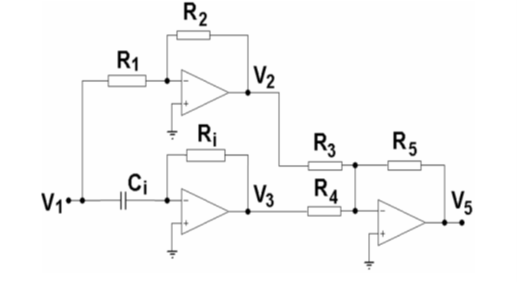
\includegraphics[width=0.7\textwidth]{pictures/topic2_a.png}
            \caption{Đề bài bài 2 hình thứ nhất}					
            \label{fig:circuit_simulation}
        \end{figure}
        \subsubsection{Tìm mối quan hệ input và output}
            \hspace*{0.6cm}Xét riêng rẻ từng mạch Opamp ta có: 
            \begin{align}
                V_{2} &= -\frac{R_2}{R_1} \cdot V_{1} \tag{1} \\
                V_{3} &= -R_{I} \cdot C_{I} \cdot \frac{dV_{1}}{dt} \tag{2} \\
                V_{out} &= -\frac{R_{5}}{R_3} \cdot V_{2} - \frac{R_{5}}{R_4} \cdot V_{3} \tag{3}
            \end{align}
            \hspace*{0.6cm}Thế (1),(2) vào (3) ta được:
            \begin{align*}
                V_{out} &= -\frac{R_{5}}{R_3} \cdot \left(-\frac{R_2}{R_1} \cdot V_{1}\right) - \frac{R_{5}}{R_4} \cdot \left(-R_{I} \cdot C_{I} \cdot \frac{dV_{1}}{dt}\right) \\
                        &= \frac{R_{5} \cdot R_2}{R_1 \cdot R_3} \cdot V_{1} + \frac{R_{5} \cdot R_{I} \cdot C_{I}}{R_4} \cdot \frac{dV_{1}}{dt}
            \end{align*}
            \hspace*{0.6cm}Đặt $A=\frac{R_{5} \cdot R_2}{R_1 \cdot R_3}$, $B=\frac{R_{5} \cdot R_{I} \cdot C_{I}}{R_4}$, ta có: $V_{out} = A \cdot V_{1} + B \cdot \frac{dV_{1}}{dt}$ \\
            \hspace*{0.6cm}Theo đề bài ta có các giá trị R, C là tự do nên ta chọn $R_{1} = R_{2} = R_{3} = R_{4} = R_{5} = 10k\Omega, R_{I} = 100k\Omega, C_{I} = 10\mu F$ $\Rightarrow A = B = 1$. \\
            \hspace*{0.6cm}Nên mối quan hệ giữa input và output là: $V_{out} = V_{1} + \frac{dV_{1}}{dt}$ \\
            \hspace*{0.6cm}Chọn dòng điện đầu vào có dạng: $V_{1} = sin(100\pi \cdot t)$ 
            \begin{align*}
                \Rightarrow V_{out} &= sin(100\pi \cdot t) + \frac{d}{dt} \left(sin(100\pi \cdot t)\right) \\
                                    &= sin(100\pi \cdot t) + 100\pi \cdot cos(100\pi \cdot t) \\
                                    &= sin(100\pi \cdot t) + 100\pi \cdot cos(100\pi \cdot t)
            \end{align*}
        \subsubsection{Kiểm tra lại bằng proteus}
            \begin{itemize}
                \item Sử dụng Proteus để mô phỏng mạch như hình: 
                \begin{figure}[H]
                    \centering
                    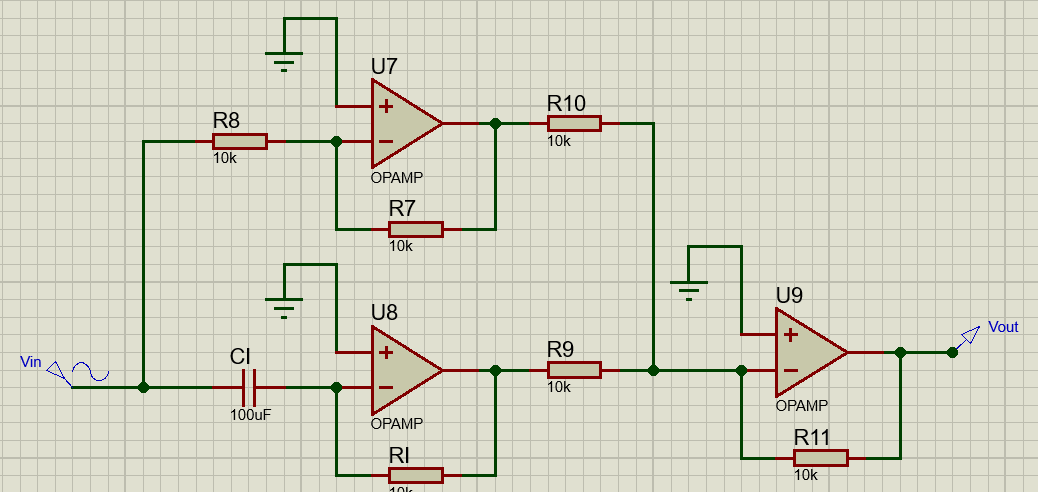
\includegraphics[width=120mm, height=80mm]{pictures/result2_a_1.png}
                    \caption{Mô phỏng proteus bài 2 hình thứ nhất}					
                \end{figure}
                \item Các linh kiện sử dụng: Opamp, Resistor, Capacitor, Voltage Source Sine, Ground.
                \item Chọn $R_{1} = R_{2} = R_{3} = R_{4} = R_{5} = 10k\Omega, R_{I} = 100k\Omega, C_{I} = 10\mu F$. $V_{1} = sin(2\pi t)$. \\
                $\Rightarrow V_{out} = sin(100\pi t) + 2\pi cos(2\pi t)$. \\
                Đặt $V_{out} = R \cdot sin{\omega t + \phi}$, với: $R = \sqrt{1^2 + (2\pi)^2} = 6.3622, \phi = \arctan(\frac{2\pi}{1}) \approx 81^\circ$.
                \item Kết quả mô phỏng proteus.
                \begin{figure}[H]
                    \centering
                    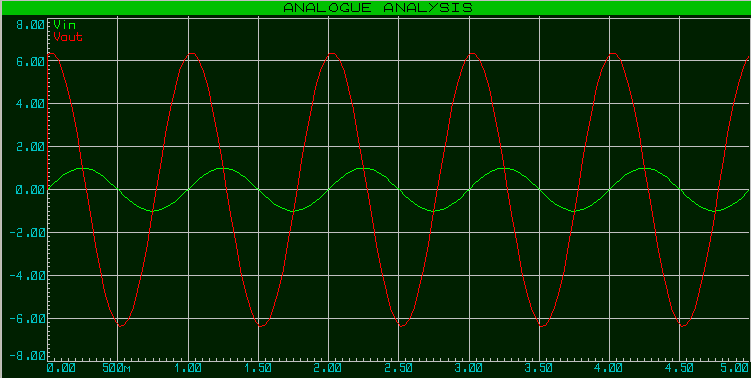
\includegraphics[width=120mm, height=80mm]{pictures/result2_a_2.png}
                    \caption{Kết quả mô phỏng proteus bài 2 hình thứ nhất}
                \end{figure}
                \item Từ kết quả so sánh giữa $V_{1}$ và $V_{out}$ ta thấy rằng $V_{out}$ trễ pha khoảng hơn $90^\circ$ so với $V_{1}$ và $V_{out}$ có giá trị cực đại khoảng $6.36$.
            \end{itemize}
            \hspace*{0.6cm}$\Rightarrow$ Kết quả mô phỏng gần đúng với tính toán.
    \subsection{Hình thứ hai}
        \begin{figure}[H]
            \centering
            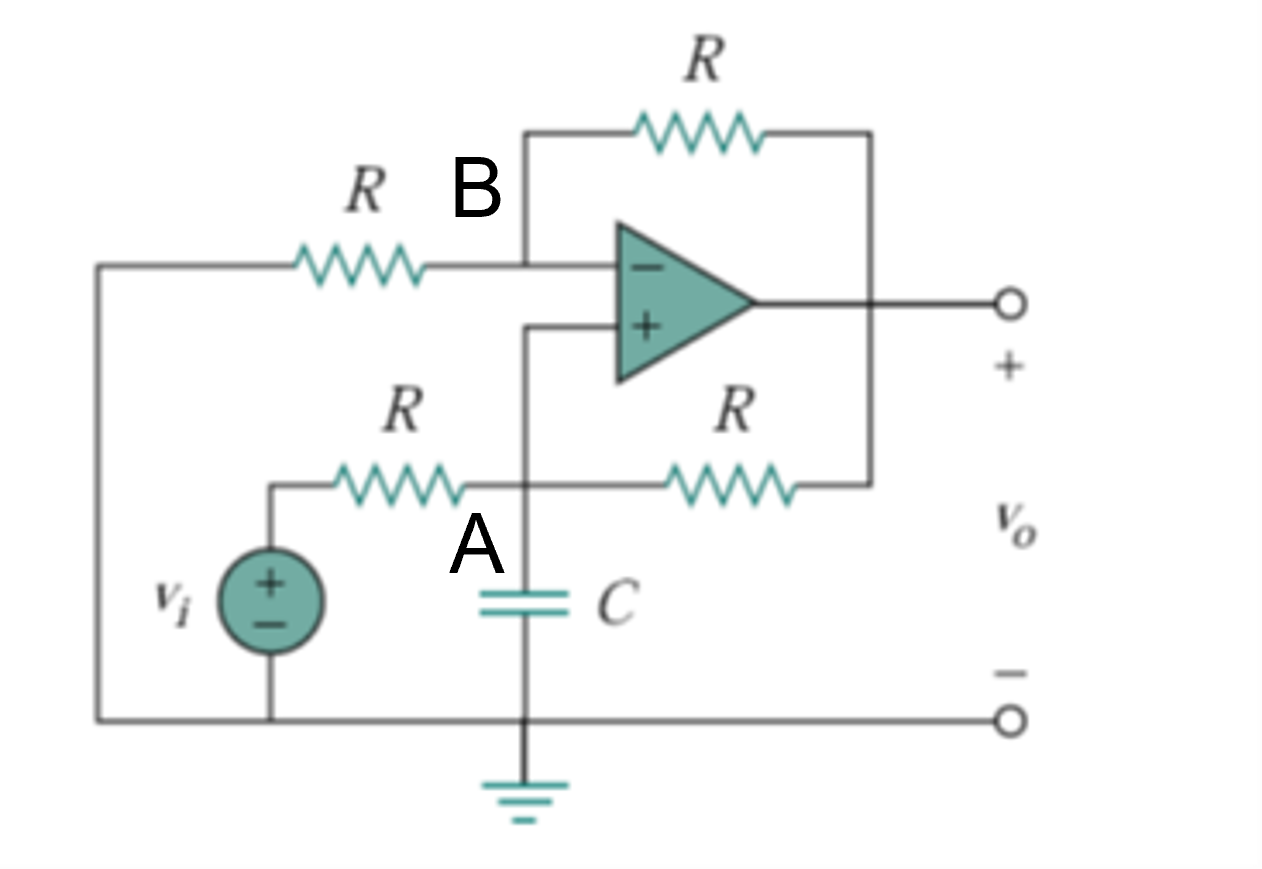
\includegraphics[width=0.7\textwidth]{pictures/topic2_b.png}
            \caption{Đề bài bài 2 hình thứ hai}					
            \label{fig:circuit_simulation}
        \end{figure}
        \subsubsection{Tìm mối quan hệ input và output}
            \hspace*{0.6cm}Giả sử KĐTT là lý tưởng, ta có:
            \[
				\begin{cases}
					I^+ = I^- = 0\\
					V_{+} = V_{-} = V\\
				\end{cases}
			\]
            \hspace*{0.6cm}Áp dụng định luật K1 đối với node B ta có: 
            \begin{align}
                \frac{V_{-}}{R} = \frac{V_{o} - V_{-}}{R} \Rightarrow V_{o}= 2V
            \end{align}
            \hspace*{0.6cm}Áp dụng định luật K1 đối với node A ta có:
            \begin{align}
                \frac{V_{in} - V_{+}}{R} = \frac{C \cdot dV_{+}}{dt} - (\frac{V_{out} - V_{+}}{R}) 
            \end{align}
            \hspace{0.6cm}Từ (7) và (8) $\Rightarrow V_{out} = \frac{2}{RC} \int V_{in} dt$ \\
        \subsection{Kiểm tra lại bằng proteus}
            \begin{itemize}
                \item Sử dụng Proteus để mô phỏng mạch như hình: 
                \begin{figure}[H]
                    \centering
                    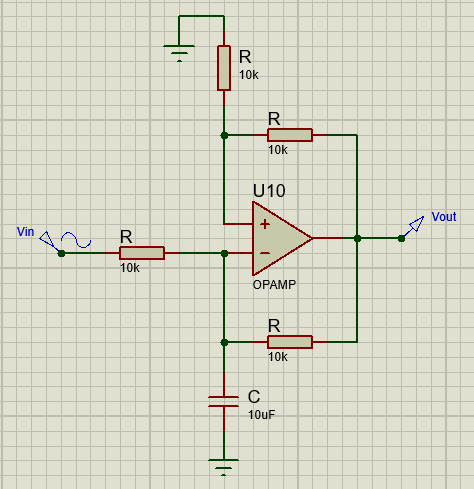
\includegraphics[width=100mm, height=90mm]{pictures/result2_b_1.png}
                    \caption{Mô phỏng proteus bài 2 hình thứ hai}					
                \end{figure}
                \item Các linh kiện sử dụng: Opamp, Resistor, Capacitor, Voltage Source Sine, Ground.
                \item Chọn $R = 10k\Omega, C = 10\mu F$. $V_{in} = 1sin(100\pi t)$. \\
                $\Rightarrow V_{out} = 20\int sin(100\pi t) dt = -\frac{20}{100\pi}cos(100\pi t) + Constant = \frac{20}{100\pi}cos(100\pi t+ pi) + Constant$.
                \item Kết quả mô phỏng proteus.
                \begin{figure}[H]
                    \centering
                    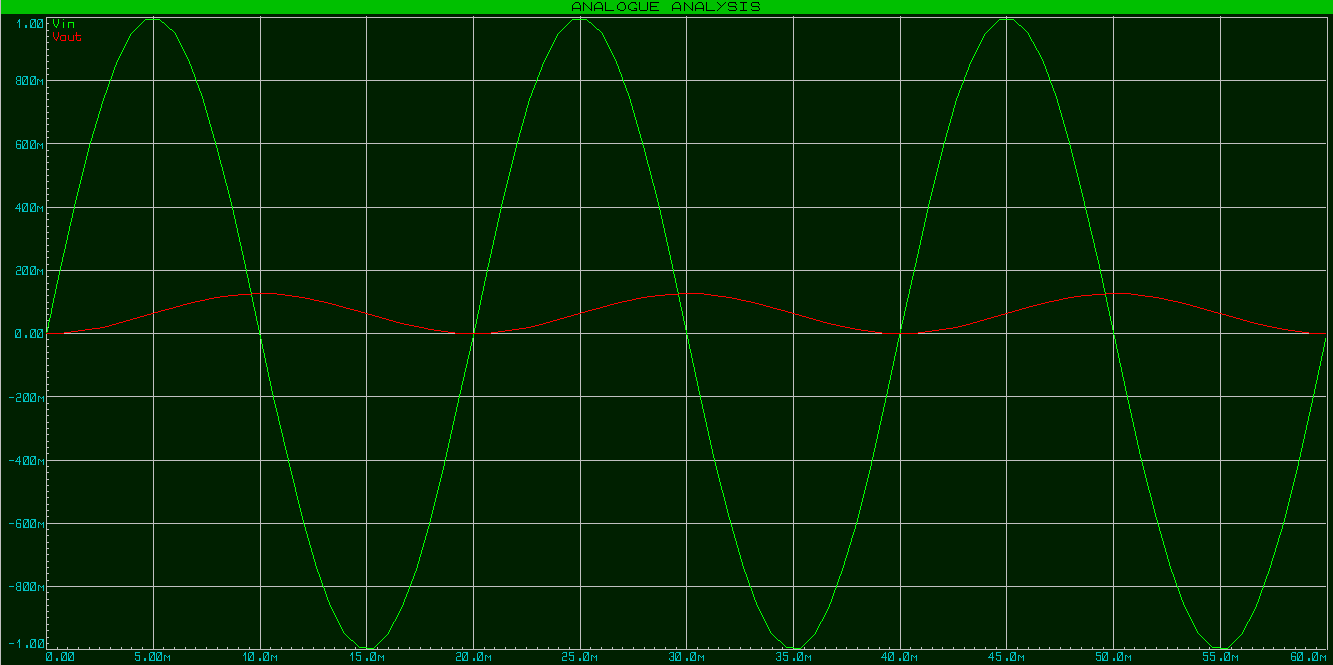
\includegraphics[width=110mm, height=80mm]{pictures/result2_b_2.png}
                    \caption{Kết quả mô phỏng proteus bài 2 hình thứ 2}
                \end{figure}
                \item Từ kết quả so sánh giữa $V_{in}$ và $V_{out}$ ta thấy rằng $V_out$ trễ pha $\pi$ so với $V_in$ và $V_out$ có khoảng dao động $L \approx 0.13$ tương ứng với 2 lần biên độ dao động điều hòa: $2 \cdot A = 2 \cdot \frac{20}{100 \pi} = 0.127$.
            \end{itemize}
            \hspace*{0.6cm}$\Rightarrow$ Kết quả mô phỏng gần đúng với tính toán.



            